% Influence of the hallway width on the success of the simulation

\begin{figure}[h!]
	\centering
		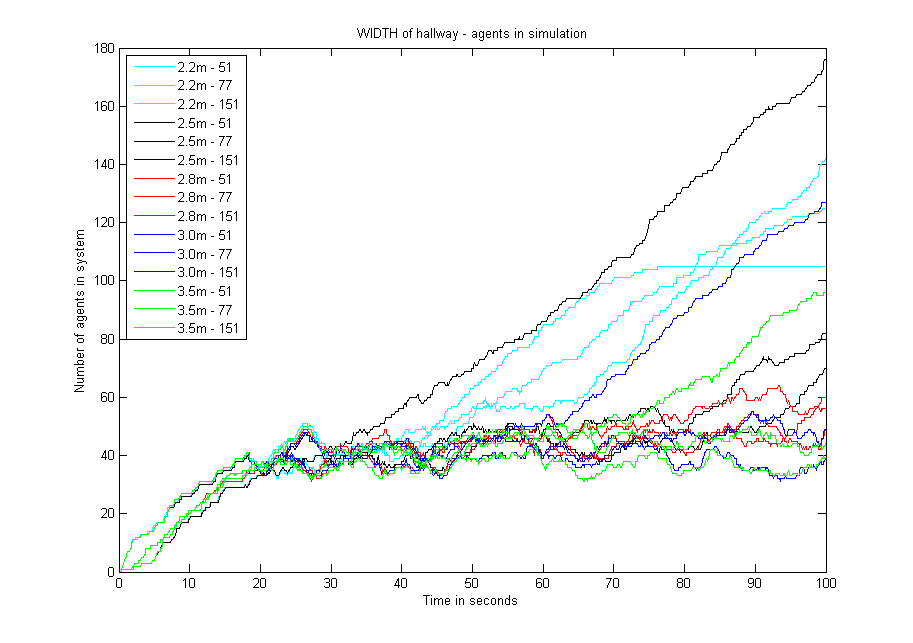
\includegraphics[width=0.90\textwidth]{pictures/AallInOne.png}
	\caption{The plot shows the total number of agents in the system for different widths and seeds in dependence of the simulation time. This number exceeds an equilibrium value (around 40-50 agents) when a jam started. To show the total agent number's dependence on the hallway width, each seed to a certain width was coloured equally. Hallway widths used were 2.2, 2.5, 2.8, 3.0 and 3.5 m. One can see here that the narrower a hallway is, the more probable jams pop up, but from 2.8 meters on it mostly worked well.}
	\label{fig:WidthAllInOne}
\end{figure}

\noi As a fast visual analysis, one can see that for 2.2 and 2.5 meters width, every simulation got stuck. Two 2.8 meters width simulations also had a jam started at the end of the simulation. In addition to those, also one of the three simulations of 3.0 and 3.5 meters width each got stuck too.\\

\noi To detect jams, looking at the total number of agents in the system was a suitable way as this number starts to increase strongly when agents start to get stuck. Figure \ref{fig:WidthAllInOne} shows the total agent number in all 15 simulations that were carried out evolving in time. What one can clearly see is that the results are not perfect and that random chance plays a big role as for example also one simulation of a 3.5 meters wide hallway started jammed even though there would have been plenty of space left at the formation of the jam.\\
But there are tendencies which are nevertheless visible: The most obvious thing is that there really is a equilibrium of people in the simulations when the simulation runs smoothly. This is where most of the graphs are. When a jam pops up, the number of agents starts to increase quite linearly because agents are spawned but can't reach the end of the hallway. The horizontal line is a clear sign that both spawn zones are clogged up.\\

\begin{figure}[h!]
	\centering
		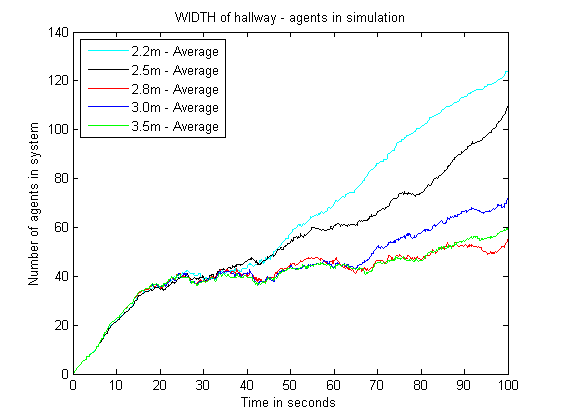
\includegraphics[width=1.00\textwidth]{pictures/AAveragesInOne.png}
	\caption{This plot shows the number of agents in the system for different widths and seeds in dependence of the simulation time. The total agent numbers of three seeds were averaged to one vector for better visibility. This number exceeds equilibrium (around 40-50 agents) when a jam started.  Hallway widths used were 2.2, 2.5, 2.8, 3.0 and 3.5 m. The total agent number's dependence on the hallway width can be seen here: The narrower a hallway is, the more probable jams pop up, but from 2.8 meters on it mostly worked well. The 3.0 m graph can be looked at as an exception because one of its seeds exploded quite badly so the average looks high too.}
	\label{fig:AveragesInOne}
\end{figure}

\noi In figure \ref{fig:AveragesInOne}, the data sets for each seeds were averaged for better visibility. One can clearly see the tendency for narrower hallways to get more jams, although the others rise up too due to the average taken over equilibrium seeds and jam seeds.\\

\noi The observed tendency was in accordance with what we expected, although we hoped for a bigger difference in the success rate.\\

To sum up, the tendencies observed in this simulation series are quite obvious: The more narrow a hallway gets, the higher the probability is to get stuck, which can be seen as all the 2.2 and 2.5 meter wide simulations ended in jams. Also, two of the 2.8 meter hallway simulations ended in jams, but for wider hallways, only coincidence made jams possible.\\
One can derive from this, that there is a certain width that will mostly work and is between 2.8 and 3.0 meters. Anything higher won't be much of an improvement for the chosen densities, because the flux is already smooth but won't be faster. But as the hallway is narrowed, jams are inevitable.\\
